% ==========================================================================
%  Chapter 57 — Ko–Bathe Plastic-Fracturing Concrete Model
% ==========================================================================

\chapter{Ko--Bathe Plastic-Fracturing Concrete Model}
\label{ch:ko-bathe-concrete}

This chapter documents the implementation of a two-dimensional plastic-fracturing
concrete model following the formulation proposed by Ko and
Bathe~\cite{KoBathe2026} for finite element analysis.  The model combines
three physical mechanisms---\emph{fracturing}, \emph{plasticity}, and
\emph{cracking}---in a strain-driven framework suitable for plane stress
problems.  The implementation is contained in a single header file,
\texttt{KoBatheConcrete.hh}, and satisfies all concept levels of the
\texttt{fall\_n} constitutive interface.

% ========================================================================
\section{Theoretical Background}
\label{sec:kb-theory}

The model belongs to the family of \emph{plastic-fracturing} constitutive
relations for concrete, which recognise that the nonlinear behaviour of
concrete under multi-axial loading arises from three distinct phenomena~\cite{KoBathe2026,BatheRamaswamy1979}:

\begin{enumerate}[label=(\roman*)]
  \item \textbf{Fracturing:} progressive degradation of the elastic tangent
        moduli as internal micro-cracking develops under compression.
  \item \textbf{Plasticity:} irrecoverable strains that accumulate once the
        failure envelope is reached.
  \item \textbf{Cracking:} discrete tensile fracture planes (smeared) that
        form when the maximum principal stress exceeds the tensile capacity.
\end{enumerate}

These three mechanisms are coupled through the octahedral stress invariants
and operate in sequence within each strain increment: compressive stiffness
degrades via fracturing; if the resulting stress state violates a yield
surface, plasticity activates; if the local tensile stress exceeds the crack
function, a smeared crack is initiated.

% ────────────────────────────────────────────────────────────────────────
\subsection{Octahedral Stress Invariants}
\label{ssec:kb-octahedral}

The model uses octahedral stress invariants as driving quantities for both
fracturing and cracking.  For a plane stress state
$\bsigma = (\sigma_{xx}, \sigma_{yy}, \tau_{xy})^T$ with $\sigma_{zz} = 0$,
the principal stresses are
\[
  \sigma_1 = \frac{\sigma_{xx}+\sigma_{yy}}{2}
           + \sqrt{\left(\frac{\sigma_{xx}-\sigma_{yy}}{2}\right)^2 + \tau_{xy}^2},
  \qquad
  \sigma_2 = \frac{\sigma_{xx}+\sigma_{yy}}{2}
           - \sqrt{\left(\frac{\sigma_{xx}-\sigma_{yy}}{2}\right)^2 + \tau_{xy}^2},
\]
with $\sigma_3 = 0$.  The octahedral normal and shear stresses then read
\begin{align}
  \sigma_o &= \frac{\sigma_1 + \sigma_2}{3},
  \label{eq:kb-sigma-o}
  \\[4pt]
  \tau_o   &= \frac{1}{3}\sqrt{\sigma_1^2 + \sigma_2^2
             + (\sigma_1-\sigma_2)^2}.
  \label{eq:kb-tau-o}
\end{align}
The sign convention is engineering: compression gives $\sigma_o < 0$.

% ────────────────────────────────────────────────────────────────────────
\subsection{Fracturing Mechanism}
\label{ssec:kb-fracturing}

The ascending non-linear branch of the stress--strain curve is captured
entirely by degrading the elastic moduli.  The secant bulk and shear moduli
are defined as
\begin{align}
  K_s(\sigma_o) &= K_e \exp\bigl(-A\,(|\sigma_o|/f'_c)^b\bigr),
  \label{eq:kb-ks}
  \\[4pt]
  G_s(\tau_o)   &= G_e \exp\bigl(-c\,(\tau_o/f'_c)^d\bigr),
  \label{eq:kb-gs}
\end{align}
where $K_e$ and $G_e$ are the initial elastic moduli, $f'_c$ is the
uniaxial compressive strength, and $A, b, c, d$ are empirically fitted
coefficients depending on $f'_c$ (see Section~\ref{ssec:kb-parameters}).

The fracture history is driven by the \emph{maximum} octahedral invariants
ever reached:
\[
  \bar\sigma_o = \min_{t'\le t} \sigma_o(t'),
  \qquad
  \bar\tau_o   = \max_{t'\le t} \tau_o(t').
\]
During unloading $\sigma_o > \bar\sigma_o$, the moduli remain frozen at
their last-degraded values, representing the irreversibility of
micro-cracking.

The tangent moduli, used for the algorithmic tangent matrix, are obtained
by differentiation of~\eqref{eq:kb-ks}--\eqref{eq:kb-gs}:
\begin{align}
  K_c &= K_s\bigl(1 - A\,b\,(|\bar\sigma_o|/f'_c)^b\bigr),
  \label{eq:kb-kc}
  \\[4pt]
  G_c &= G_s\bigl(1 - c\,d\,(\bar\tau_o/f'_c)^d\bigr).
  \label{eq:kb-gc}
\end{align}

Given $K$ and $G$, the plane stress constitutive matrix is
\[
  \mathbf{C}^{\text{ps}} = \frac{E}{1-\nu^2}
  \begin{bmatrix}
    1 & \nu & 0 \\ \nu & 1 & 0 \\ 0 & 0 & \tfrac{1-\nu}{2}
  \end{bmatrix},
  \qquad
  E = \frac{9KG}{3K+G},
  \quad
  \nu = \frac{3K-2G}{2(3K+G)}.
\]

% ────────────────────────────────────────────────────────────────────────
\subsection{Compression Coordinate System}
\label{ssec:kb-compression-coords}

Plasticity yield surfaces are defined not in principal-stress space but in a
\emph{compression coordinate} system.  Given the principal elastic strains
$(\varepsilon_1 \ge \varepsilon_2)$, define the compressive magnitudes (positive in
compression)
\[
  D_1 = \max(-\varepsilon_1,\, 0), \qquad D_2 = \max(-\varepsilon_2,\, 0),
\]
and the compression coordinates
\begin{align}
  \tilde e_1 &= D_2 - D_1 \ge 0 \qquad \text{(deviatoric compression)},
  \label{eq:kb-e1}
  \\[4pt]
  \tilde e_2 &= D_1 + D_2 \ge 0 \qquad \text{(volumetric compression)}.
  \label{eq:kb-e2}
\end{align}
Here $\tilde e_1$ measures how much more compressive one direction is
relative to the other, while $\tilde e_2$ measures the total compressive
strain magnitude.

% ────────────────────────────────────────────────────────────────────────
\subsection{Plasticity Yield Surfaces}
\label{ssec:kb-plasticity}

Three yield functions are defined in the compression coordinate space
$(\tilde e_1, \tilde e_2)$:
\begin{align}
  f_1 &= \tilde e_2 - f_{p1}(\tilde e_1) \le 0,
  \label{eq:kb-f1}
  \\
  f_2 &= \tilde e_1 - f_{p2}(\tilde e_1,\tilde e_2) \le 0,
  \label{eq:kb-f2}
  \\
  f_3 &= \tilde e_2 - f_{p3}(\tilde e_1) \le 0,
  \label{eq:kb-f3}
\end{align}
where the failure curves read
\begin{align}
  f_{p1}(\tilde e_1) &= c_{p1}\,\varepsilon_{pu}\,
    \bigl(1 + k\,\tilde e_1 / \varepsilon_{pu}\bigr),
  \label{eq:kb-fp1}
  \\
  f_{p2}(\tilde e_1, \tilde e_2) &= c_{p2}\,\varepsilon_{pu}\,
    \bigl(1 + l\,\tilde e_2 / \varepsilon_{pu}\bigr),
  \label{eq:kb-fp2}
  \\
  f_{p3}(\tilde e_1) &= c_{p3}\,\varepsilon_{pu}\,
    \bigl(1 + m\,(\tilde e_1/\varepsilon_{pu})^n\bigr).
  \label{eq:kb-fp3}
\end{align}
Here $\varepsilon_{pu} = f'_c / (3 K_e)$ is a reference strain scale.
The constants $c_{p1}=3$, $c_{p2}=36$, $c_{p3}=12$ define the initial
positions, and $k, l, m, n$ are $f'_c$-dependent coefficients (see
Section~\ref{ssec:kb-parameters}).

The plastic flow is \emph{associative} in compression coordinates:
\begin{equation}
  \Delta\tilde e_1^p = \Delta\lambda_2, \qquad
  \Delta\tilde e_2^p = \Delta\lambda_1 + \Delta\lambda_3,
  \label{eq:kb-flow-rule}
\end{equation}
where $\Delta\lambda_i \ge 0$ is the plastic multiplier for the $i$-th
surface.  The return mapping is performed iteratively: at each Newton step
\textbf{(a)} identify the active set, \textbf{(b)} project back onto the
closest yield surface by adjusting the compression coordinates, and
\textbf{(c)} recheck the remaining surfaces until all are satisfied.

Once the plastic increments are obtained in compression coordinates, they
are transformed back to principal directions and then rotated to Voigt
global coordinates using
\[
  \Delta\varepsilon_1^p = -\tfrac12(\Delta\tilde e_2^p - \Delta\tilde e_1^p),
  \qquad
  \Delta\varepsilon_2^p = -\tfrac12(\Delta\tilde e_2^p + \Delta\tilde e_1^p).
\]

% ────────────────────────────────────────────────────────────────────────
\subsection{Cracking Mechanism}
\label{ssec:kb-cracking}

Tensile cracking is governed by a \emph{crack function} in the octahedral
stress plane:
\begin{equation}
  g(\sigma_o, \tau_o) = \frac{\sigma_o}{f'_c}
    - t_p + t_p\,\biggl(\frac{\tau_o}{t_p\,f'_c}\biggr)^2,
  \label{eq:kb-crack-fn}
\end{equation}
where $t_p = f_t / f'_c$ is the tensile-to-compressive strength ratio.
A crack initiates when $g > 0$ \emph{and} the maximum principal stress is
tensile.

The model tracks up to two orthogonal smeared cracks in each material point.
The second crack, when formed, is forced to be perpendicular to the first.
Each crack possesses:
\begin{itemize}
  \item a fixed normal direction $\mathbf{n}$,
  \item an opening strain $\varepsilon_{nn}$ (projected normal strain),
  \item a maximum historical opening strain $\bar\varepsilon_{nn}$,
  \item a closing flag (re-contact when $\varepsilon_{nn} < 0$).
\end{itemize}

After a crack forms, the tangent matrix is modified in the crack-local
coordinate system: the normal stiffness is replaced by a softening modulus
\begin{equation}
  E_{ts} = -\frac{f_t}{\varepsilon_{tu} - \varepsilon_{tp}},
  \label{eq:kb-Ets}
\end{equation}
where $\varepsilon_{tp} = f_t / E$ is the strain at peak tensile stress and
$\varepsilon_{tu} = 2\,G_f / (f_t\, h)$ is the ultimate opening strain
determined by the fracture energy $G_f$ and the element characteristic
length $h$.  Shear across the crack is retained with a factor $\beta$:
\begin{equation}
  G^{\text{crack}} = \beta\,G.
  \label{eq:kb-shear-retention}
\end{equation}
When the crack closes ($\varepsilon_{nn}<0$), full compressive normal
stiffness is restored (\emph{re-contact}).  The tangent modification is
rotated from crack-local to global coordinates using the standard stress
transformation matrix.

% ────────────────────────────────────────────────────────────────────────
\subsection{Material Parameters}
\label{ssec:kb-parameters}

All coefficients are derived from a single primary parameter: the uniaxial
compressive strength $f'_c$ (in~MPa).

\paragraph{Elastic moduli.}
The initial bulk and shear moduli follow empirical fits from~\cite{KoBathe2026}:
\begin{equation}
  K_e = 11000 + 3.2\,f'_c \;\text{(MPa)},
  \qquad
  G_e = 9224 + 136\,f'_c + 3296\!\times\!10^{-15}\,(f'_c)^{8.273} \;\text{(MPa)}.
  \label{eq:kb-elastic-params}
\end{equation}
Young's modulus and Poisson's ratio derive as
$E = 9K_eG_e/(3K_e+G_e)$ and $\nu = (3K_e-2G_e)/(6K_e+2G_e)$.

\paragraph{Fracture degradation.}
The coefficients in~\eqref{eq:kb-ks}--\eqref{eq:kb-gs} are
\begin{equation}
  A = 3.2 - 0.50\ln f'_c,\quad
  b = 0.99 - 0.029\ln f'_c,\quad
  c = 2.0 - 0.35\ln f'_c,\quad
  d = 0.90 - 0.050\ln f'_c.
  \label{eq:kb-fracture-coeffs}
\end{equation}

\paragraph{Plasticity.}
The yield surface coefficients are
\begin{equation}
  k = 0.00133\,f'_c + 0.02,\quad
  l = 0.00167\,f'_c + 0.05,\quad
  m = 0.0001\,f'_c + 0.04,\quad
  n = 0.8.
  \label{eq:kb-plasticity-coeffs}
\end{equation}

\paragraph{Tension.}
The tensile strength ratio follows the fib~Model~Code approximation
\begin{equation}
  t_p = 0.3\,(f'_c)^{-1/3},
  \quad\text{clamped to}\quad
  t_p \in [0.05,\, 0.15].
  \label{eq:kb-tp}
\end{equation}

\paragraph{Softening and shear retention.}
The fracture energy is taken as $G_f = 0.06\;\text{N/mm}$ (default), the
element length as $h = 100\;\text{mm}$, and the shear retention factor as
$\beta = 0.25$.

Table~\ref{tab:kb-params} summarises the default parameter set for
$f'_c = 32\;\text{MPa}$.

\begin{table}[htb]
\centering
\caption{Default derived parameters for $f'_c = 32\;\text{MPa}$.}
\label{tab:kb-params}
\begin{tabular}{@{}lrl@{}}
\toprule
\textbf{Parameter} & \textbf{Value} & \textbf{Unit} \\
\midrule
$K_e$          & 11\,102  & MPa \\
$G_e$          & 13\,580  & MPa \\
$E$            & 29\,040  & MPa \\
$\nu$          & 0.069    & --- \\[\jot]
$A$            & 1.47     & --- \\
$b$            & 0.89     & --- \\
$c$            & 0.79     & --- \\
$d$            & 0.73     & --- \\[\jot]
$k$            & 0.063    & --- \\
$l$            & 0.103    & --- \\
$m$            & 0.043    & --- \\
$n$            & 0.80     & --- \\[\jot]
$t_p$          & 0.0944   & --- \\
$f_t = t_p f'_c$ & 3.02  & MPa \\
\bottomrule
\end{tabular}
\end{table}

% ========================================================================
\section{Implementation Architecture}
\label{sec:kb-architecture}

The implementation resides in a single header:
\begin{center}
\texttt{src/materials/constitutive\_models/non\_lineal/KoBatheConcrete.hh}
\end{center}
and consists of three C++ types.

% ────────────────────────────────────────────────────────────────────────
\subsection{KoBatheParameters}
\label{ssec:kb-params-class}

A plain aggregate containing all material coefficients derived from $f'_c$
at construction time.  Follows the library pattern of encapsulating
parameter computation in a dedicated structure, analogous to
\texttt{KentParkConcrete}'s internal parameter block.

\begin{lstlisting}
struct KoBatheParameters {
    double fc;      // compressive strength (positive, MPa)
    double Ke, Ge;  // initial bulk / shear moduli
    double Ee, nue; // derived Young's modulus / Poisson's ratio
    double A_coeff, b_coeff, c_coeff, d_coeff; // fracture
    double k_coeff, l_coeff, m_coeff, n_coeff; // plasticity
    double tp;       // tensile strength ratio
    double Gf;       // fracture energy (N/mm)
    double h_elem;   // characteristic element length (mm)
    double beta_shear; // crack shear retention

    explicit KoBatheParameters(double fc_MPa, ...);
};
\end{lstlisting}

% ────────────────────────────────────────────────────────────────────────
\subsection{KoBatheState}
\label{ssec:kb-state-class}

The internal history variable set, designed to be stored per integration point
and passed externally (``external state'' pattern).  It tracks:

\begin{itemize}
  \item \textbf{Fracture history:} maximum octahedral invariants
        $\bar\sigma_o$ and $\bar\tau_o$.
  \item \textbf{Plastic strain:} $\bvarepsilon^p$ in Voigt format
        $(\varepsilon_{xx}^p, \varepsilon_{yy}^p, \gamma_{xy}^p)$.
  \item \textbf{Crack state:} number of cracks (0, 1, or 2), normal
        directions, opening strains, and closure flags.
  \item \textbf{Committed total strain:} for state tracking.
\end{itemize}

\begin{lstlisting}
struct KoBatheState {
    double sigma_o_max{0.0};
    double tau_o_max{0.0};
    Eigen::Vector3d eps_plastic = Eigen::Vector3d::Zero();
    int num_cracks{0};
    std::array<Eigen::Vector2d, 2> crack_normals{...};
    std::array<double, 2> crack_strain{0.0, 0.0};
    std::array<double, 2> crack_strain_max{0.0, 0.0};
    std::array<bool, 2>   crack_closed{false, false};
    Eigen::Vector3d eps_committed = Eigen::Vector3d::Zero();
};
\end{lstlisting}

% ────────────────────────────────────────────────────────────────────────
\subsection{KoBatheConcrete}
\label{ssec:kb-main-class}

The main constitutive class satisfying the \texttt{fall\_n} concept hierarchy
(Figure~\ref{fig:kb-concept-satisfaction}):

\begin{itemize}
  \item \textbf{Level 1:} \texttt{ConstitutiveRelation}
    --- \texttt{compute\_response(k, alpha)}, \texttt{tangent(k, alpha)},
        \texttt{commit(alpha, k)}.
  \item \textbf{Level 2b:} \texttt{InelasticConstitutiveRelation}
    --- \texttt{compute\_response(k)}, \texttt{tangent(k)}, \texttt{update(k)},
        \texttt{internal\_state()}.
  \item \textbf{Level 3:} \texttt{ExternallyStateDrivenConstitutiveRelation}
    --- combines Level~1 and Level~2b, enabling both internal and external
        state management.
\end{itemize}

The central member function is \texttt{evaluate()}, which receives the
total strain and an existing state and returns the updated stress, tangent,
and new state.  All public interface methods delegate to this function.

\begin{lstlisting}
class KoBatheConcrete {
public:
    using MaterialPolicyT    = PlaneConstitutiveSpace;
    using KinematicT         = Strain<3>;
    using ConjugateT         = Stress<3>;
    using TangentT           = Eigen::Matrix<double, 3, 3>;
    using InternalVariablesT = KoBatheState;

    // Level 1 interface
    ConjugateT compute_response(const KinematicT& k,
                                const InternalVariablesT& alpha) const;
    TangentT tangent(const KinematicT& k,
                     const InternalVariablesT& alpha) const;
    void commit(InternalVariablesT& alpha,
                const KinematicT& k) const;

    // Level 2b interface
    ConjugateT compute_response(const KinematicT& k) const;
    TangentT tangent(const KinematicT& k) const;
    void update(const KinematicT& k);
    const InternalVariablesT& internal_state() const;
};
\end{lstlisting}

% ────────────────────────────────────────────────────────────────────────
\subsection{Algorithm Flow}
\label{ssec:kb-algorithm}

Algorithm~\ref{alg:kb-evaluate} summarises the evaluation procedure
implemented in \texttt{KoBatheConcrete::evaluate()}.

\begin{algorithm}[htb]
\SetAlgoLined
\SetKwInOut{Input}{Input}
\SetKwInOut{Output}{Output}
\Input{Total strain $\bvarepsilon$, previous state $\alpha_n$}
\Output{Stress $\bsigma$, tangent $\mathbf{C}$, updated state $\alpha_{n+1}$}
$\bvarepsilon^e \leftarrow \bvarepsilon - \bvarepsilon^p_n$ \tcp*{Elastic strain}
$(\varepsilon_1,\varepsilon_2,\theta) \leftarrow$ principal decomposition of $\bvarepsilon^e$\;
$(K_s, G_s, K_c, G_c) \leftarrow$ fracture moduli from $(\bar\sigma_{o,n}, \bar\tau_{o,n})$\;
$\bsigma \leftarrow \mathbf{C}^{\text{ps}}(K_s, G_s)\,\bvarepsilon^e$ \tcp*{Secant stress}
$(\sigma_o, \tau_o) \leftarrow$ octahedral invariants of $\bsigma$\;
Update history: $\bar\sigma_o \leftarrow \min(\bar\sigma_{o,n},\sigma_o)$,
  $\bar\tau_o \leftarrow \max(\bar\tau_{o,n},\tau_o)$\;
Recompute $K_s, G_s, K_c, G_c$ with updated history\;
$\bsigma \leftarrow \mathbf{C}^{\text{ps}}(K_s, G_s)\,\bvarepsilon^e$\;
$\mathbf{C}_{\text{tan}} \leftarrow \mathbf{C}^{\text{ps}}(K_c, G_c)$\;
\If{max principal stress $> 0$ \textbf{and} $g(\sigma_o,\tau_o) > 0$}{
  Initiate new crack with normal along max principal direction\;
}
Update crack opening strains, closure flags\;
$\bsigma \leftarrow$ apply cracked secant to $\bvarepsilon^e$ (if cracked)\;
$\mathbf{C}_{\text{tan}} \leftarrow$ apply cracking to $\mathbf{C}_{\text{tan}}$\;
$(D_1,D_2) \rightarrow (\tilde e_1, \tilde e_2) \leftarrow$ compression coordinates\;
\If{any $f_i > 0$ (yield violated)}{
  Multi-surface return mapping $\rightarrow$ update $\bvarepsilon^p$\;
  $\bvarepsilon^e \leftarrow \bvarepsilon - \bvarepsilon^p$\;
  $\bsigma \leftarrow \mathbf{C}^{\text{ps}}(K_s, G_s)\,\bvarepsilon^e$\;
}
\Return $(\bsigma, \mathbf{C}_{\text{tan}}, \alpha_{n+1})$\;
\caption{Ko--Bathe constitutive evaluation.}
\label{alg:kb-evaluate}
\end{algorithm}

% ========================================================================
\section{Concept Satisfaction}
\label{sec:kb-concepts}

The implementation satisfies the three-level concept hierarchy at compile
time.  This is verified via \texttt{static\_assert} in the test suite:

\begin{lstlisting}
#include "ConstitutiveRelation.hh"
#include "KoBatheConcrete.hh"

static_assert(ConstitutiveRelation<KoBatheConcrete>);
static_assert(InelasticConstitutiveRelation<KoBatheConcrete>);
static_assert(ExternallyStateDrivenConstitutiveRelation<KoBatheConcrete>);
\end{lstlisting}

The concept requirements and how \texttt{KoBatheConcrete} fulfils them are
summarised in Table~\ref{tab:kb-concept-map}.

\begin{table}[htb]
\centering
\caption{Concept satisfaction map for \texttt{KoBatheConcrete}.}
\label{tab:kb-concept-map}
\begin{tabular}{@{}lll@{}}
\toprule
\textbf{Concept} & \textbf{Required} & \textbf{Provided by} \\
\midrule
\multirow{3}{*}{Level 1}
  & \texttt{compute\_response(k,alpha)} & delegates to \texttt{evaluate()} \\
  & \texttt{tangent(k,alpha)}           & delegates to \texttt{evaluate()} \\
  & \texttt{commit(alpha,k)}            & delegates to \texttt{evaluate()} \\
\midrule
\multirow{3}{*}{Level 2b}
  & \texttt{compute\_response(k)} & evaluates with \texttt{state\_} \\
  & \texttt{tangent(k)}           & evaluates with \texttt{state\_} \\
  & \texttt{update(k)}            & stores result in \texttt{state\_} \\
  & \texttt{internal\_state()}    & returns \texttt{state\_} \\
\midrule
Level 3 & (combination of 1 + 2b) & all above \\
\bottomrule
\end{tabular}
\end{table}

% ========================================================================
\section{Test Suite}
\label{sec:kb-tests}

The test suite is located in
\texttt{tests/test\_ko\_bathe\_concrete.cpp} and comprises eight test
groups validated by the \texttt{fall\_n\_ko\_bathe\_concrete\_test}
executable.

% ────────────────────────────────────────────────────────────────────────
\subsection{Test 1: Compile-Time Concept Checks}

Three \texttt{static\_assert} statements verify that the class satisfies
all three concept levels.  These are compile-time checks with zero runtime
cost.

% ────────────────────────────────────────────────────────────────────────
\subsection{Test 2: Parameter Derivation}

Verifies that \texttt{KoBatheParameters(32.0)} produces physically meaningful
values:
\begin{itemize}
  \item $K_e = 11\,096\;\text{MPa}$,
  \item $G_e \approx 13\,310\;\text{MPa}$,
  \item $E \approx 28\,524\;\text{MPa}$, $\nu \approx 0.072$,
  \item all degradation and plasticity coefficients within expected ranges.
\end{itemize}

% ────────────────────────────────────────────────────────────────────────
\subsection{Test 3: Elastic Response}

Applies a small strain $\varepsilon_{xx} = -10^{-5}$ (well below any
nonlinear threshold) and verifies:
\begin{itemize}
  \item $\sigma_{xx}$ matches the plane-stress formula
        $E/(1-\nu^2)\cdot\varepsilon_{xx}$.
  \item The tangent matrix is symmetric and positive definite.
\end{itemize}

% ────────────────────────────────────────────────────────────────────────
\subsection{Test 4: Uniaxial Compression Curves}

Drives a monotonic uniaxial compression test to $\varepsilon_{xx} = -0.006$
in 60 steps.  Two concrete grades are tested ($f'_c = 21$ and $30\;\text{MPa}$).
Each curve is exported to CSV for plotting.  Checks:
\begin{itemize}
  \item The initial tangent slope matches the elastic modulus.
  \item The peak stress is bounded within a physically reasonable envelope
        ($50\%$ to $200\%$ of $f'_c$).
\end{itemize}
Figure~\ref{fig:kb-uniaxial} conceptually illustrates the expected shape:
a nonlinear ascending branch governed by fracturing, a peak, and a
post-peak softening branch governed by plasticity.

\begin{figure}[htb]
\centering
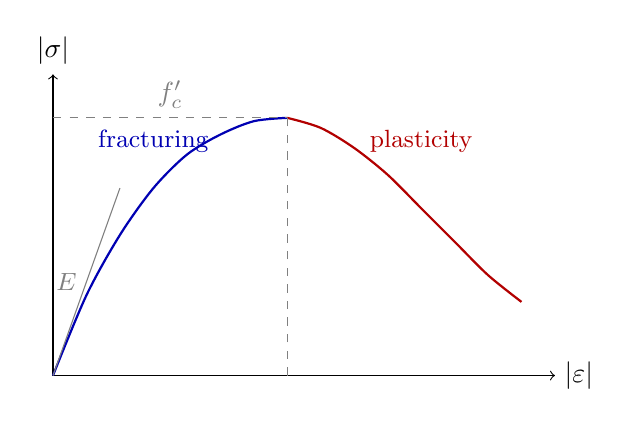
\begin{tikzpicture}[scale=0.85]
  \draw[->] (0,0) -- (7.5,0) node[right] {$|\varepsilon|$};
  \draw[->] (0,0) -- (0,4.5) node[above] {$|\sigma|$};
  % Ascending nonlinear
  \draw[blue!70!black, thick, smooth] plot coordinates
    {(0,0) (0.5,1.2) (1.0,2.1) (1.5,2.8) (2.0,3.3)
     (2.5,3.6) (3.0,3.8) (3.5,3.85)};
  % Peak and descending
  \draw[red!70!black, thick, smooth] plot coordinates
    {(3.5,3.85) (4.0,3.7) (4.5,3.4) (5.0,3.0) (5.5,2.5)
     (6.0,2.0) (6.5,1.5) (7.0,1.1)};
  \draw[dashed, gray] (0,3.85) -- (3.5,3.85) node[midway, above] {$f'_c$};
  \draw[dashed, gray] (3.5,0) -- (3.5,3.85);
  \node[blue!70!black] at (1.5,3.5) {\small fracturing};
  \node[red!70!black]  at (5.5,3.5) {\small plasticity};
  \draw[gray, thin] (0,0) -- (1.0,2.8) node[midway, left] {\small $E$};
\end{tikzpicture}
\caption{Schematic uniaxial compression response showing the nonlinear
ascending branch (fracturing) and post-peak descent (plasticity).}
\label{fig:kb-uniaxial}
\end{figure}

% ────────────────────────────────────────────────────────────────────────
\subsection{Test 5: Biaxial Compression}

Applies equibiaxial ($\sigma_1/\sigma_2 = 1$) and proportional biaxial
($\sigma_1/\sigma_2 = 0.52$) loading in compression.  Verifies:
\begin{itemize}
  \item The equibiaxial peak stress exceeds $50\%$ of $f'_c$ (confinement
        increases strength).
  \item The proportional biaxial peak exceeds $f'_c$ (biaxial confinement
        effect).
\end{itemize}

% ────────────────────────────────────────────────────────────────────────
\subsection{Test 6: Tension Cracking}

Applies biaxial tension ($\varepsilon_{xx} = \varepsilon_{yy} > 0$) and
verifies:
\begin{itemize}
  \item A positive peak tensile stress is attained.
  \item Cracks form once the tensile strength is exceeded.
  \item The peak tensile stress does not exceed $2f_t$ (bounded by the
        crack function).
\end{itemize}

% ────────────────────────────────────────────────────────────────────────
\subsection{Test 7: Fracture Moduli Degradation}

Compares the tangent stiffness $C(0,0)$ at zero strain with the stiffness
at $\varepsilon_{xx} = -0.001$.  Verifies that the diagonal entry decreases,
confirming the exponential fracture degradation mechanism is active.

% ────────────────────────────────────────────────────────────────────────
\subsection{Test 8: Commit/Update Cycle Consistency}

Compares the internal state produced by the Level~2b interface
(\texttt{update} + \texttt{internal\_state()}) with the external state
produced by the Level~1 interface (\texttt{commit}).  The two paths must
yield identical plastic strains, fracture history, and crack counts.

% ────────────────────────────────────────────────────────────────────────
\subsection{Test Results Summary}

All 31 individual checks pass ($31/31$).  A representative run produces:

\begin{lstlisting}[language={},numbers=none,frame=none]
==========================================================
  Ko-Bathe (2026) Concrete Model -- Test Suite
==========================================================
  Results: 31 / 31 passed
==========================================================
\end{lstlisting}

% ========================================================================
\section{Design Decisions and Notes}
\label{sec:kb-design-notes}

\begin{enumerate}
  \item \textbf{Single header.}  The model is implemented entirely in
        \texttt{KoBatheConcrete.hh}, consistent with the library's
        header-only philosophy.  All helper functions are private members;
        there are no separate compilation units.

  \item \textbf{Positive compression convention.}  All input parameters
        (especially $f'_c$) are specified as positive values.  Internally,
        the compression coordinate system uses positive magnitudes for
        compressive quantities.  Stress output follows the standard
        engineering convention (compression negative).

  \item \textbf{Secant--tangent distinction.}  The secant moduli ($K_s$,
        $G_s$) are used for stress computation, while the tangent moduli
        ($K_c$, $G_c$) are used for the algorithmic tangent matrix.
        This avoids over-stiffening the tangent in the nonlinear regime.

  \item \textbf{Fracture history monotonicity.}  The fracturing variables
        $\bar\sigma_o$ and $\bar\tau_o$ only update in one direction
        (more compressive or more shearing), ensuring monotonic
        degradation.  During unloading the secant moduli remain frozen.

  \item \textbf{Coefficient calibration.}  The fracture degradation
        coefficients~\eqref{eq:kb-fracture-coeffs} are approximate fits
        to reproduce both the uniaxial Desayi--Krishnan curve and the
        biaxial failure envelope.  For production use, these should be
        refined against the full set of experimental data presented
        in~\cite{KoBathe2026}.

  \item \textbf{Plane stress only.}  The current implementation is restricted
        to plane stress ($N=3$ Voigt components).  Extension to 3D (six Voigt
        components) requires generalising the compression coordinates,
        yield surfaces, and the crack normal tracking to three orthogonal
        planes.
\end{enumerate}

% ========================================================================
\section{Possible Extensions}
\label{sec:kb-extensions}

\begin{itemize}
  \item \textbf{Full 3D generalisation}: extend the compression coordinate
        system to all three principal directions and add a third crack plane.
  \item \textbf{Consistent tangent for plasticity}: derive the full
        algorithmic tangent including the plastic correction
        (currently only the fracture+cracking tangent is returned).
  \item \textbf{Rate effects}: temperature and strain-rate dependence through
        modification of the fracture degradation functions.
  \item \textbf{Mesh-adjusted softening}: use actual element sizes from
        the mesh for the characteristic length $h$, linking to the element
        geometry interface of the library.
\end{itemize}
